
\begin{minipage}[top]{10cm}
L'entreprise est à la recherche de qualifications de plus en plus élevées pour faire face au développement de technologies en constante évolution et pour une bonne compréhension des consignes de travail. Lors de sa scolarité, un jeune doit développer de l'intérêt et de la curiosité, si utiles pour réussir ensuite sa vie professionnelle. Face au nombre, en baisse mais encore inquiétant, de sorties du système scolaire sans qualification, il paraît intéressant d'étudier ce phénomène du point de vue européen à la lumière des mathématiques. En France, 13\% des jeunes de 18 à 24 ans qui ne poursuivent pas d'études ni de formation n'ont ni CAP, ni BEP, ni bac et sont sortants précoces.
\end{minipage}
\begin{minipage}{6cm}
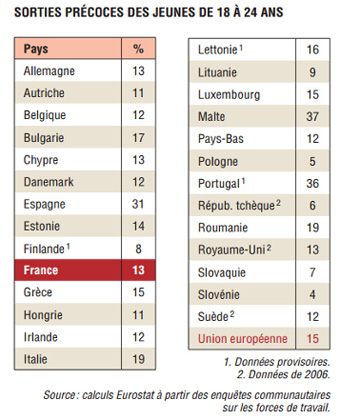
\includegraphics[scale=0.5]{stat12.jpg} 
\end{minipage}

\begin{enumerate}
\item Calculer la moyenne des sorties précoces en Europe à l'aide des données du tableau. Que remarquez-vous ? Justifier.
\item Tracer une représentation graphique de ce tableau sur tableur ou sur une feuille.
\item Compléter le tableau suivant et construire l'histogramme de cette série.

\begin{tabular}{|c|c|c|c|c|c|c|}
\hline 
Sorties précoces en 2007 & [0;5[ & [5;10[ & [10;15[ & [15;20[ & [20;25[ & [25;30] \\ 
\hline 
Nombre de pays européens &  &  &  &  &  &  \\ 
\hline 
\end{tabular} 

\item Calculer la moyenne des sorties précoces en Europe à l'aide de la question 3. Comparer le résultat avec la question 1.  
\end{enumerate}




  